
\documentclass{article}[12pt]
%Required: You must have these
\usepackage{graphicx}
\usepackage{tabularx}
\usepackage{natbib}
%\usepackage{caption}
%\usepackage{subcaption}
\usepackage{array}
\usepackage{amsmath}
%\usepackage[backend=bibtex]{biblatex}
\setkeys{Gin}{width=0.8\textwidth}
%\setlength{\captionmargin}{30pt}
\setlength{\abovecaptionskip}{10pt}
\setlength{\belowcaptionskip}{10pt}
\topmargin -1.5cm 
\oddsidemargin -0.04cm 
\evensidemargin -0.04cm 
\textwidth 16.59cm
\textheight 23.94cm 
\parskip 7.2pt 
\renewcommand{\baselinestretch}{1.1} 	
\parindent 0pt

\bibliographystyle{refs/styles/newphyto.bst}
\usepackage{Sweave}
\begin{document}
\Sconcordance{concordance:prief_manuscript.tex:prief_manuscript.Rnw:1 187 1}


% emw13Jun -- Hi - hi! I know this in super draft mode, but made some notes on the text. I hope that is okay. If it is too soon, just delete them and skip reading them. 

\section{Introduction}
Each spring, in ecosystems across the temperate zone, ecological communities re-assemble form their period of winter dormancy with the hatching of insects, arrival of migratory birds, the germination of seeds and emergence of new leaves and flowers. The phenology---or seasonal timing---of these re-occurring life cycle events can be quite different, even among closely related organism in a shared habitat \citep{}. There is growing evidence that these phenological differences among taxa play a major role in dictating community interactions and shaping the structure and function of ecological communities \citep{}.

% emw13Jun -- I would draw out the below paragraph some, maybe a short paragraph on seasonal priority effects, giving empirical examples of how they may structure communities. Then a new paragraph on how this has led to growing interest in the role of seasonal priority effects in coexistence, that focuses on model results and ends on climate change (as you introduce these a little be sure to focus on TIMING or some word that hints at this being different than phenology). Also, I think we'll need more time to walk readers through types of competitive ability more slowly -- if you get in first and draw the resource, then under some scenarios you are the better competitor and a lot of readers will think that, but here we use competitive ability as competitive ability under low resource conditions. I wonder if we could get away with skipping this discussion (and effectively any discussion of the trade-off) until after the 'recent work on models' section below? We could just hint at here then, something like 'growing interest... new models ... many suggest timing as fundamental to coexistence with several suggesting a fundamental trade-off between being early for early, priority access to resources versus being later but competing well under low resource conditions.'
Phenological differences among species can generate seasonal priority effects; when earlier active species gain a competitive advantage by accesses limiting resources before their competitors emerge or arrive and modifying the environment that later emerging species experience \citep{}. Studies in plants \citep{}, insects \citep{}, birds \citep{} and mammals \citep{} have found that even small phenological priority effects, on the order of just a few days, can substantially alter competitive hierarchies in ways that can persist across several growing seasons \citep{}.

The demonstrated importance of seasonal priority effects in mediating interspecific competition has led to growing interest in the role of seasonal priority effects in coexistence \citep{Diez_2024, Blackford_2020}. Several existing community assembly models that integrate the timing of species arrive or activity suggest timing is fundamental to coexistence---with several studies suggesting there is a fundamental trade-off between early phenology to gain unrestricted access to finite resources versus later later phenology, but competing well under low resource conditions \citep{}. But the interest in understanding seasonal priority effects also highlights one of the major challenges to the field: phenology is not a static trait but varies across years as it is the realized product of an interaction between the environment (cues) and species unique physiology and genetic and developmental attributes \citep{}.

Environmental cues are changing rapidly, in fact phenological, shifts are one of the most pronounced indicators of climate change to date \citep{}. However species' phenological responses to climate change differ significantly. We suggest that the degree to which a species responds to environmental variation known as \textbf{phenological sensitivity} ($\Delta$ phenology/ $\Delta$ environmental cue) is the primary mediator of the tradeoff between phenology and competition, and understanding this trait is key to predicting community assembly in an era of global change. Below we outline why integrating phenological sensitivity into community assembly is critical and outline a path to develop a more robust way to predict assembly that in a rapidly changing world. 


\section{How phenological differences arise}
Environmental cues such as temperature, light and moisture are the primary triggers that control phenology \citep{}. Many species respond to multiple aspects of cues. For example, some seeds respond to light levels and daylength \citep{}, and many temperate plants require require both exposure to cool winter temperature (0-4$\degree$C, hereafter: winter chilling) and warm spring temperatures to initiate phenological activity \citep{}. These sensitivities are the unique product of species physiology, genetics and development. For example, seeds have different kinds of dormancy \citep{}. Plants and animals may relay on different cues \citep{}. What this means is that phenology itself is a response to the environment, so that \emph{realized phenology differences} between species will vary substantially depending on the environmental conditions.

% emw13Jun -- this could be much shorter and in the middle we may want to also focus on variation in germination spread maybe. I also still don't think you need the trade-off yet. You could just say: we see here that who is first depends on environmental conditions and switches year to year, yet this is not how most coexistence models approach phenology.' [then go to next section]
We illustrate this point by re-analyzing seed phenology data from \citep{}(Buonaiuto \& Wolkvich, see extended Methods for details), in which 11 co-occuring species were germinated under varying temperature conditions. We can see that even species from a common environment have very different sensitives to temperature cues (Figure \ref{Fig:germination}a). As seen in our comparison of two species, \emph{Persicaria virginiana} and \emph{Eurybia divaricata}---a pair of woodland herbs that frequently compete in Eastern Temperate Forests \citep{}---we see here that who is first depends on environmental conditions and switches with increasing cue levels. This illustrates that the strength of seasonal priority effect is highly dependent on the environment, yet this is not how most coexistence models approach phenology.


\section{Recent work integrating phenology into assembly models} % Lizzie asks: Do we want to mainly say coexistence models or assembly models or something else? Do we want to discuss `timing' here or use 'phenology' and then say -- but wait, is it phenology? 

% The widespread and obvious shifts in phenology with continued anthropogenic climate change have led to growing interest in how phenology may structure communities, with a number of models positing a correlation between timing and competition \citep{volkerisaj,wolkovich2021phenological,levine2022competition}. These models ...

Growing interest in how phenology may structure communities has led to increased modeling efforts, with most approaches centering on the relationship between timing and competition \citep{volkerisaj,wolkovich2021phenological,levine2022competition}. 
% Alternative [replace next 3-4 sentence -- until the sentence that starts `Models have done this through an...' -- with just this one sentence]: 
Building off experimental \citep{godoy2014} and observational \citep{wolkovich2013} evidence that earlier species appear to perform better models have generally built in trade-off where species with a timing advantage also experience greater competition. 
%Superficially, phenological differences may seem to promote coexistence through niche differences---if species can perfectly partition a growing season such that they never compete together. In reality, however, limited resources often confer a fitness advantage to early-species via priority access to resources or otherwise create fitness hierarchies amongst species. Thus, adding phenological variation to species in coexistence models alone is generally destabilizing and requires additional variation that effectively reduces the competition between species to stabilize such communities \citep{mcpeek2022coexistence}.
Models have done this through an explicit connection of phenological differences to parameters controlling the strength of competition \citep{volkerisaj}, or implicitly by providing a fitness advantage to earlier species that then must be offset in communities where species also vary in parameters related to $R^*$ \citep{wolkovich2021phenological,levine2022competition}.
% All models are variations on Lotka-Volterra competition I believe: \citep{wolkovich2021phenological,levine2022competition} is $R^*$ competition while \citep{volkerisaj} is Beverton-Holt. 

These models have all recognized the importance of environmental variability in communities structured in part by phenological differences, generally including interannual variation in the environment that in turn drives differences in phenology. Many models---focused often on grasslands and water competition---have assigned phenology as equivalent to an intrinsic species-level timing (or season length strategy).  Year to year variation in the environment then alters absolute differences between species, which then consistently co-varies with resource competition \citep{godoy2014,levine2022competition}. In these approaches the relative orders between species remain fixed, but other models allow species relative orders and timings to vary year-to-year assuming the underlying relationship between pairwise differences in timings and interspecific-competition is known---and static. % These models thus fix the relationship between phenology and interspecific-competition.
Each of these approaches in turn thus fixes one aspect of environment $\times$ phenology $\times$ competition relationship, an understandable simplification, but one that may make forecasting community shifts with climate change challenging. 

Community assembly models including phenology have all included environmental variability \citep{volkerisaj,levine2022competition} assuming an underlying stationary environment (one that varies year-to-year but with an underlying constant distribution), but climate change represents a clearly non-stationary environment. Temperature, for example, trends higher in its mean over time, with potential additional changes to the variance \citep{ipcc2021}. Because environmental variability in assembly models structures what species combinations are stable, shifts in the environment with anthropogenic climate change are likely to reshape communities, but forecasting them requires accurately capturing how the environment affects phenology and competition together in the simplest---but still robust---form. We argue this means capturing how dynamically the environment can determine both absolute and relative timings of species, and the how those timings directly impact co-existence. While current modeling approaches to date have simplified one aspect of this problem, it can be tractably addressed through new models that explicitly allow these dynamics in both inter- and inter-annual time, and connect to the underlying physiology of phenology. 

% Few studies have included non-stationarity environments as they violate most analytical modeling assumptions \citep{chessonnonstat}, but simulation results suggest an environment shifting to earlier growing seasons could reduce destabilize exiting communities \citep{wolkovich2021phenological}. 

% Most models have ... simplified species phenologies (to ignore the germination kernel? To make phenology inttrinsic?)  % models have all generally treated timing as an intrinsic species trait ...except that \citep{volkerisaj} allows species to flip in order between years. 

\section{Climate Change, Phenology and Coexistence}
Extending community assembly models to encapsulate the strong inter-dependence between environmental variability, phenological variability and variability competition strength, highlights that for any species that currently coexist due to the tradeoff between relative phenology and intrinsic competitive ability, climate change will disrupt this coexistence mechanism. In extending a traditional assembly models to include phenological sensitivity in it's simplest form (two species with differential sensitivity to one environmental cue), we found that no species that coexist under one climate condition through this mechanism can continue to coexist in the other (Figure \ref{Fig:differences}a). This is because the relative phenological differences between species that structures the tradeoff are dependent on and interaction between each species' phenological sensitivity and the environment itself, and therefore, the relationship between phenological sensitivity differences and realized phenological differences shift between environments (Figure \ref{Fig:differences}b).

Our modeling extension reveal an additional, critical point for improving the predictive power of coexistence model with climate change. While tradeoff between realized phenological differences and competitive differences is stable across a shifting environment, it is the tradeoff between phenological sensitivity differences and competition differences (Figure \ref{Fig:differences}a,c). It is better characterizing this tradeoff between phenological sensitivity and competition differences that should be the focus of future model development.

.%DMB I am trying to tie back to the ideas two paragraphs ago where we say all other models fix one of these aspects.
%Species all have this sort of variation, so may use to inherently bet hedge within years and between years in important ways that other models miss. Building in phenology as and then something about the shifting environment and how we need to know that too -- the species cue system and how the environment shifts (this could then hint at the future empirical directions would be nice to interweave with the modeling section here if we can.)

%Building on this physiological basis of what determines realized phenology can help us better understand how communities may shift with climate change. Species with high phenological sensitivities will benefit more from adaptive cue shifts but be more compromised by negative cue shifts than less sensitive species, but the full result depends on what stabilizes the community to begin with. If the community is assembled via some aspect of phenology, then a shifting environment could reshape that. 

%Depending on whether communities encounter and average of 6 or 12 weeks of chilling (Figure \ref{Fig:differences}a), the relationship between phenological sensitivity differences and realized phenological differences shifts (Figure \ref{Fig:differences}c), resulting in different differences (Figure \ref{Fig:differences}b) %reorder. 
%Because the fundamental tradeoff between realize phenological differences and resource competitive differences does not change in the between environments (Figure \ref{Fig:coexistence}a), the altered expression of phenology under each environments neccisitates you have different communities depending on 6 or 12 weeks (Figure \ref{Fig:coexistence}a, circled example points). (Now feeling not sure if we need figure 3b). 


%\subsection{Climate change alters relationship between phenological sensitivity and realized phenology differences}

%First to understand the effects of climate change on realized phenological differences between competing species, we ran our model under two climate change scenarios; one with a mean winter chilling period of 12 weeks and one with a winter chilling period of 6 weeks (Figure \ref{Fig:differences}a). With 12 weeks of winter chilling, the differences in realized germination phenology of compete species was minimized, with realized phenological differences being less than 2 days in approximately 50\% of model runs (Figure \ref{Fig:differences}b). Exposure to only an average 6 week of winter chilling increased the realized phenological differences between competing species with only about 10\% of of model runs producing differences in realized germination phenology of less than 2 days (Figure \ref{Fig:differences}b). % should find better, more quantitative ways to describe these differences, but for now I am just eye balling it.

%The phenological sensitives of species were drawn from the same distribution under each scenario, so the shift in realized phenological differences must be a product of the interaction between cliamte and phenological sensitivty. In fact, we see that the relationship between phenolgical sensitivity differences and realized phenological differences shifts in assoicated with the changed climate, with the slope of the relationship becoming steeper under 6 weeks of chilling (put in parameters here; Figure \ref{Fig:differences}c). Some transition statement or phrase. Next we must consider how this shift affects the tradeoff between phenology and competition.

%\subsection{Climate change alters the tradeoff between phenological sensitivity and competition}
%Because of the strong dependency on the environment and the observed shift in the relationship between phenological sensitivity and realized phenology under each climate scenario, we would expect that this shifting enviroment would alter aspects of the trade off between phenology and competition, but exactly how is not neccisarily straight forward.

%First, we find the fundamental tradeoff between realize phenological differences and competitive differences does not change in the new environment (Figure \ref{Fig:coexistence}a). This is not surprising, since the degree that phenological can offset competitive differences in fixed (say better). However, while in our models we treat inherant competition differences as fixed, it is important to note that the shift in environment changes the phenological differences of virtually all species pairs in our simulation, which means those that coexisted under one set of environmental conditions cannot coexist in a new environment, as highlighted in the circled points in Figure \ref{Fig:coexistence}a. So while the fundamental relationship between realized phenology and competitive ability doesn't change with climate change, the species that can coexist do (say better).

%Because phenological sensitivity is the mediator between environmental variation and realized phenology, the tradeoff between sensitivity differences and competitive difference must shift in accordence with the environment to maintain the realized phenolgical differences that produce coexistence. In fact we see that under 6 weeks of chilling, the slope of this relationship become steeper (put in slope value here, Figure \ref{Fig:coexistence}b), because larger differences in competitive ability are necessary to maintain the trade off in Figure \ref{Fig:coexistence}a. %% This explanation could use lots of work

% emw13Jun -- I think weaving in ecological implications as we sneak in our results throughout this section could work (I think) but we should discuss Monday if there is time about how to do it to see if we really think it would work [update 18Jun -- I am not sure our model predicts more phylogenetically distinct species co-occur ... it also has a ton of communities co-occurring because they are identical. I would focus more on the idea that traits will change or the interaction between germination timing and spread/fraction]. 
%Paragraph discussing ecological implications? eg. While our simulations are highly simplified version of a real ecological community, we can make some predictions about the kinds of species that will coexist under a novel climate. More phylogenetically distinct. Different life hystory, dormancy types. Maybe this is too hand wavy.

\section{Paths Forward}
Predicting assembly in an era of global change will require the closer integration of the kinds of physiological experiments that quantify species-level phenological sensitivity and theory \citep{recent rudolph paper}.%

Understanding how shifting environments reshape trade-offs with timing may be especially tractable in grassland systems that have been studied for this topic, but will require new data and approaches to deal with the challenges of quantifying phenological sensitivity to multiple climate cues, which increasing evidence suggests are often interactive \citep{}. Physiological studies of seed germination highlight the complexity of dealing with multiple the dimensions of temperature, light and moisture cues that affect germination timing, and how little we know about these physiological responses outside of model organisms, crops and agricultural weeds. \citep{}. Additionally, even with a better characterization of phenological response to the environment, community assembly forecasts must be filter it through how the environment is actually, changing which varies across time and space. For example. chilling goes both ways, while photoperiod doesn't change.

Selection for interacting cues is generally thought to be driven by another component likely critical for better predictions---environmental risk. Complex cues are expected to reduce risk. A reliance on winter chilling and/or photoperiod reduce the risk of frost damange in unstable spring environments). Yet few studies have formally tested this [that I know of]---a major gap that needs to be addressed for modeling. Further, ecological models generally subsume such risks into species traits (e.g., increasing maintenance costs or such), which misses the reality that such risks are a product of timing x environment.

A changing risk landscape may be the underlying driver of observed correlations between the timing and intensity component of life cycle transitions. For example, environmental cues not only influence the timing of seed germination but also the fraction of seed from any given cohort will germinate \citep{}. This basically creates additional tradeoff axes of coexistence, and would allow investigators to assess the relative importance of within season and across season bet-hedging.

Another paragraph about risk and bet hedging, and connect it back to competition.


The modeling framework we present in this study has the flexibility to be further extended to do all this (multiple cues, add risk, within and across season stuff). To make these predictions meaningful for the moment, modellers and physiologists must work together to further develop models with biologically acurate physiological processes and experiments that are readily translatable into model parameterization and development


\section*{Figures}

\begin{figure}[h!]
  \centering
 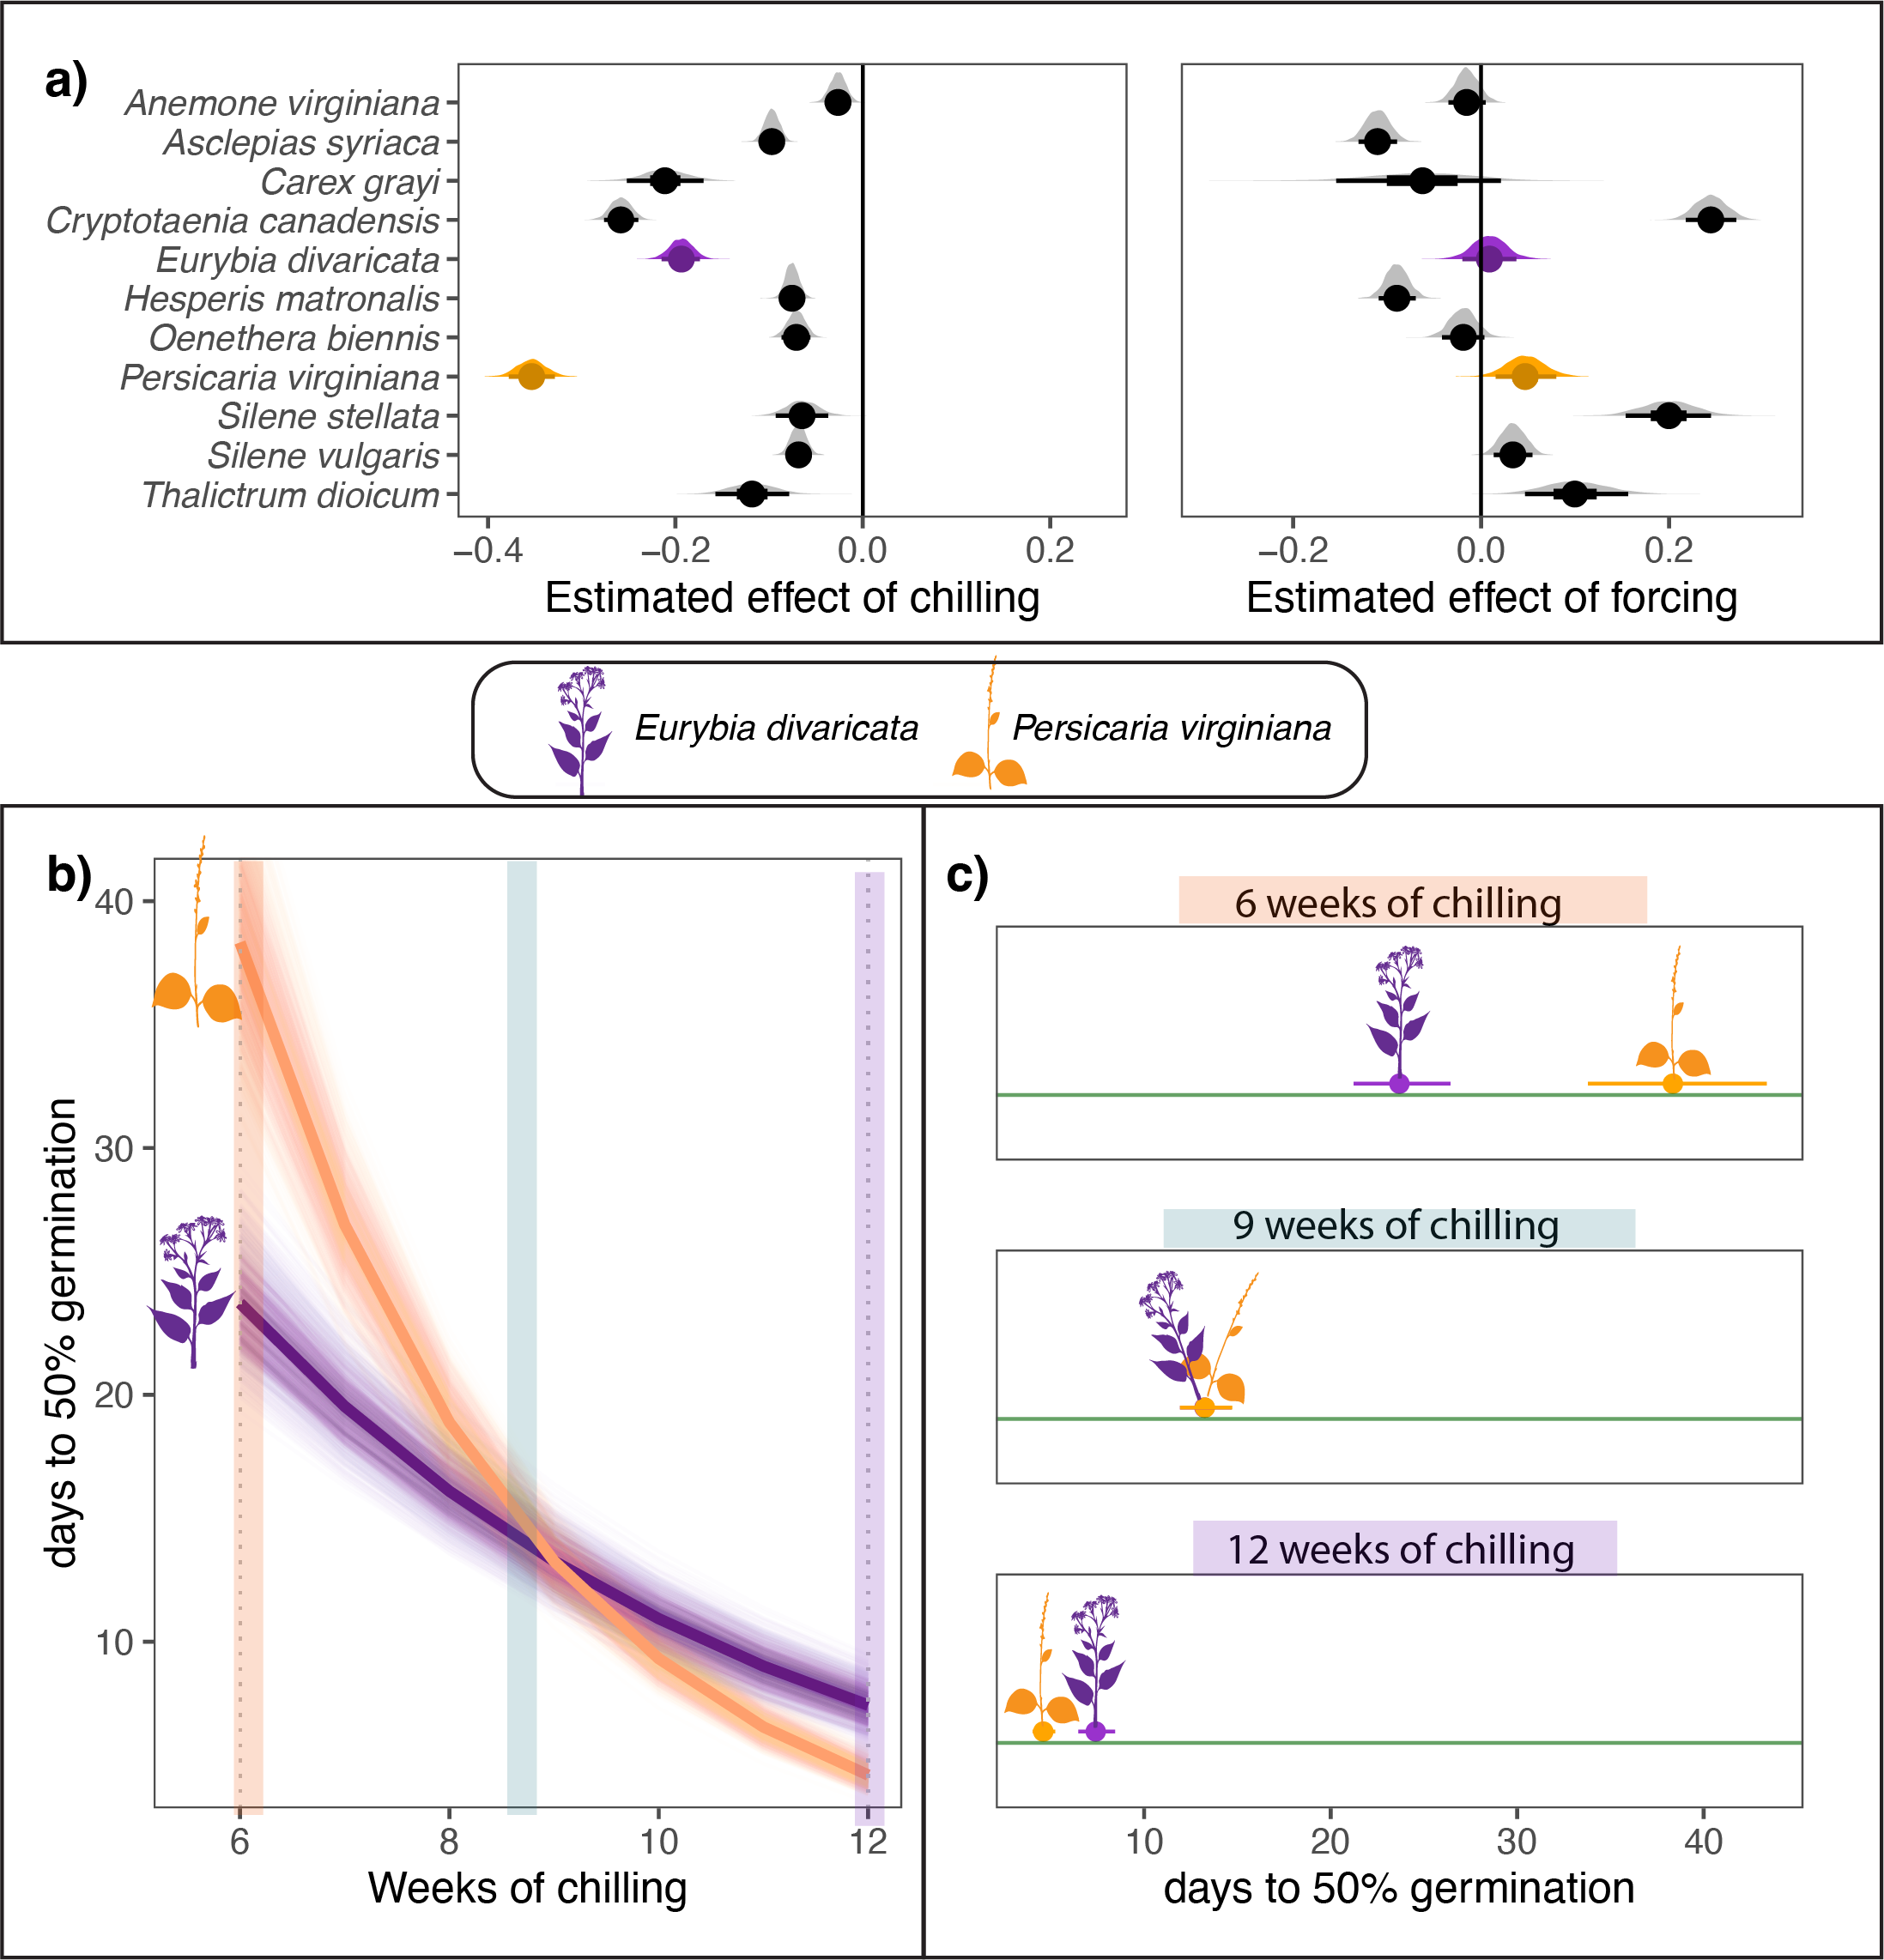
\includegraphics[width=\textwidth]{..//plots/prief_conception.png}
    \caption{\textbf{Co-occur species can differ substantially in their phenological sensitivity ($\Delta$ phenological event/$\Delta$ climate) to the environment.} Panel a) estimates the phenological sensitivity of germination timing to winter chilling and spring forcing for eleven herbaceous species of eastern North America. Points represent the mean estimate and thick and thin bars represent the 50 and 95\% uncertainty intervals. In b) and c) we highlight the phenological sensitivity to winter chilling of two species \emph{Eurybia divaricata} and \emph{Persicaria virginiana} that are commonly observed in competition. b) Depicts the sensitivity of each species to winter chilling, with thick lines representing the mean estimate and lighter lines representing modeled uncertainty. Panel c) illustrations how the species' different sensitivities manifest in contrasting realized germination differences under different climate conditions. Point represent the predicted mean number of days to 50\% germination and bars the 95\% uncertainty intervals}}. %Under six weeks of chilling \emph{E. divaricata} germinates well before \emph{P. virginiana}. Under nine weeks of chilling the species germination at roughly the same time, and under twelve weeks of chilling \emph{P. virginiana} is the first to germinate.}
    \label{Fig:germination}
\end{figure}

\begin{figure}[h!]
 \centering
 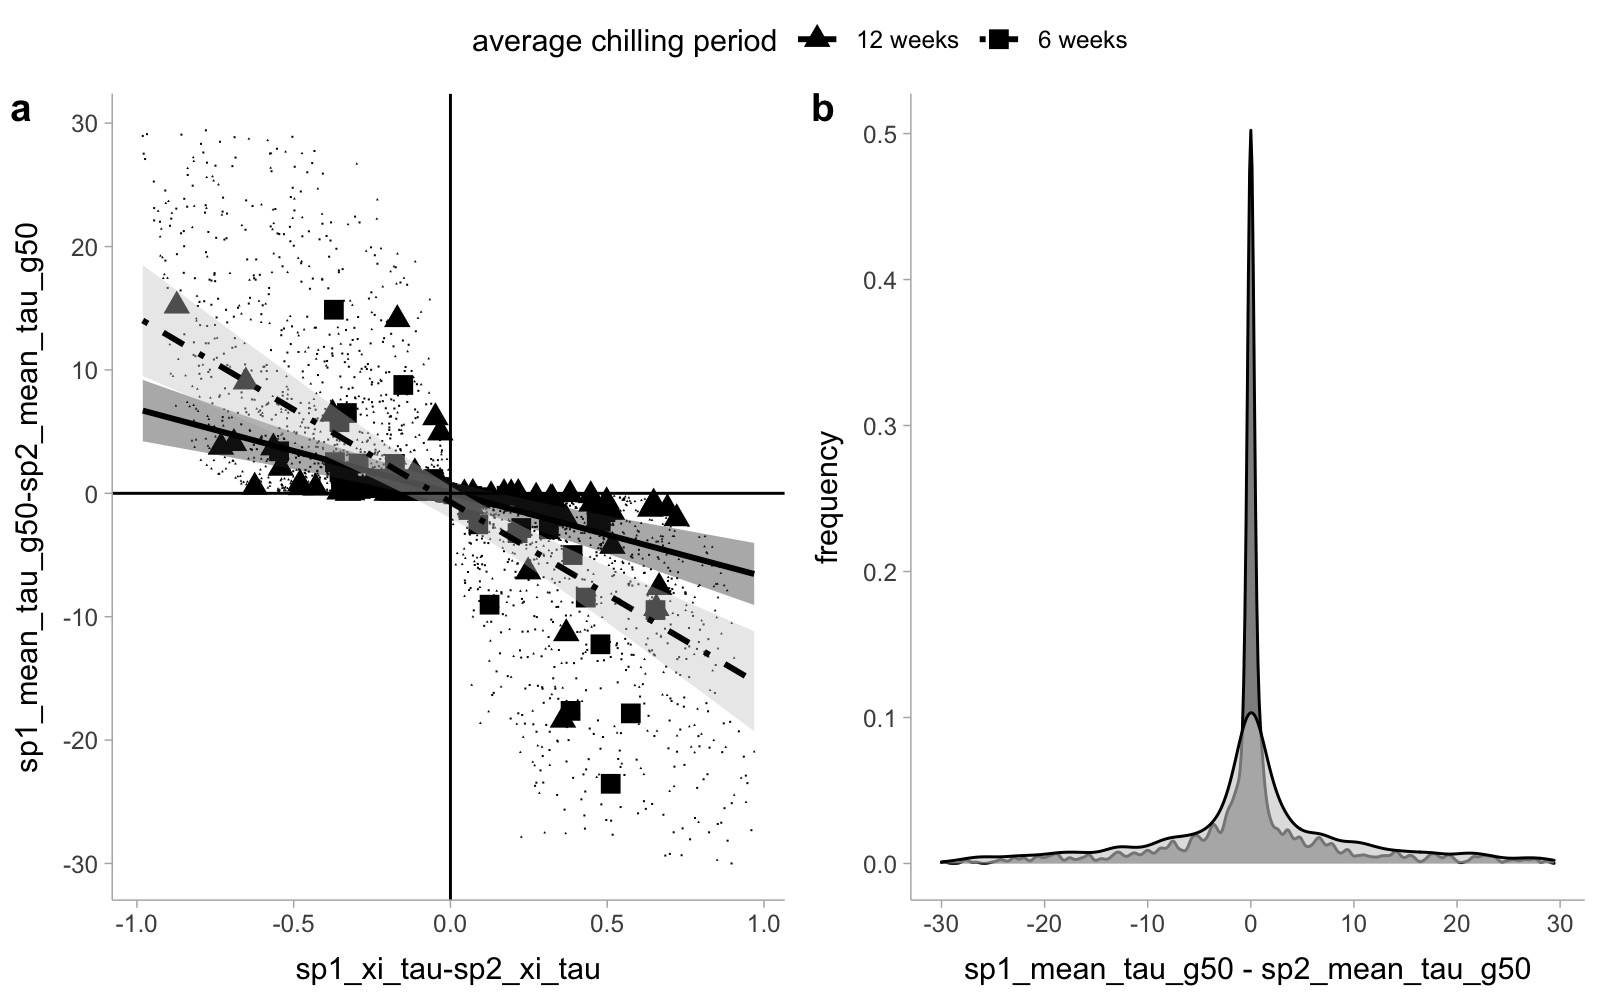
\includegraphics[width=\textwidth]{..//plots/coexistance_explainer.jpeg}
   \caption{\textbf{Climate change will the relationship phenological sensitivity differences and realized phenological differences.} Panel a) shows how climate change will shift the distribution of the duration of chilling ecological communities receive each winter. Panel b) shows the frequency distributions for the average difference in realized germination phenology under both climate scenarios---shorter chilling durations result in larger realized phenological differences between species. These changes occur because the relationship between phenological sensitivity differences and realized phenology differences, depicted in panel c), are dependent on the environment, and a change in chilling conditions alters this relationship.}
    \label{Fig:differences}
\end{figure}

\begin{figure}[h!]
  \centering
 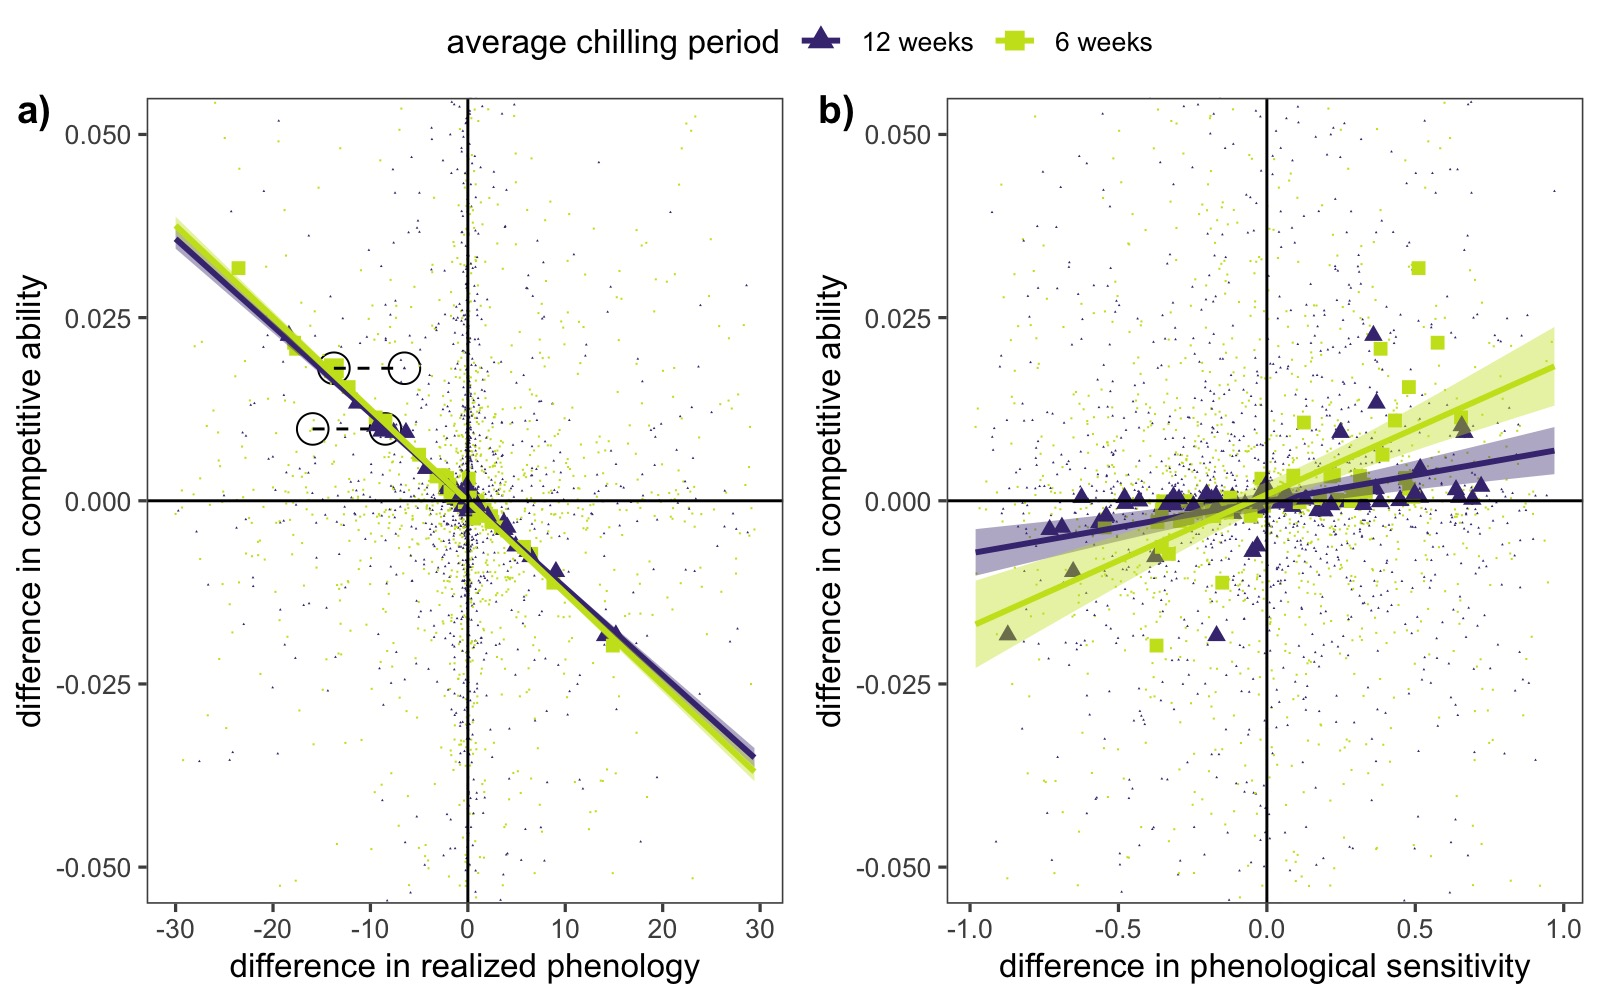
\includegraphics[width=\textwidth]{..//plots/coexistance_runner_new.jpeg}
    \caption{\textbf{Climate change will alter the relationship competititive ability, phenological sensitivty, realized phenology and coexistence.} Panel a) depicts the trade-off between realize phenological differences and competitive differences. While the tradeoff relationship between realized phenology and competition does not shift with climate change, species that coexisted under one climate scenario will not coexist if climate conditions shift, as highlighted by the two sets species pairs circled in panel a).  Panel b) depicts the trade-off between phenological sensitivity differences and competitive differences under two climate scenarios (average of 12 and 6 weeks of chilling). With climate change, the trade-off between phenological sensitivity and competition does shift because less chilling amplifies the realized phenological differences among species}
    \label{Fig:coexistence}
\end{figure}

\end{document}
